%%%%%%%%%%%%%%%%%%%%%%%%%%%%%%%%%%%%%%%%%
% baposter Portrait Poster
% LaTeX Template
% Version 1.0 (15/5/13)
%
% Created by:
% Brian Amberg (baposter@brian-amberg.de)
%
% This template has been downloaded from:
% http://www.LaTeXTemplates.com
%
% License:
% CC BY-NC-SA 3.0 (http://creativecommons.org/licenses/by-nc-sa/3.0/)
%
%%%%%%%%%%%%%%%%%%%%%%%%%%%%%%%%%%%%%%%%%

%----------------------------------------------------------------------------------------
%	PACKAGES AND OTHER DOCUMENT CONFIGURATIONS
%----------------------------------------------------------------------------------------

\documentclass[a0paper,portrait]{baposter}

\usepackage[font=small,labelfont=bf]{caption} % Required for specifying captions to tables and figures
\usepackage{booktabs} % Horizontal rules in tables
\usepackage{relsize} % Used for making text smaller in some places

\usepackage{floatrow}
\newfloatcommand{capbtabbox}{table}[][\FBwidth]
\usepackage{blindtext}
\usepackage{listings}
\usepackage{textcomp}

\usepackage{url}

\graphicspath{{figures/}} % Directory in which figures are stored

\definecolor{bordercol}{RGB}{40,40,40} % Border color of content boxes
\definecolor{headercol1}{RGB}{186,215,230} % Background color for the header in the content boxes (left side)
\definecolor{headercol2}{RGB}{80,80,80} % Background color for the header in the content boxes (right side)
\definecolor{headerfontcol}{RGB}{0,0,0} % Text color for the header text in the content boxes
\definecolor{boxcolor}{RGB}{186,215,230} % Background color for the content in the content boxes

\begin{document}
\lstset{language=SQL}

\background{ % Set the background to an image (background.pdf)
\begin{tikzpicture}[remember picture,overlay]
\draw (current page.north west)+(-2em,2em) node[anchor=north west]
{
\includegraphics[height=1.1\textheight]{background}};
\end{tikzpicture}
}

\begin{poster}{
grid=false,
borderColor=bordercol, % Border color of content boxes
headerColorOne=headercol1, % Background color for the header in the content boxes (left side)
headerColorTwo=headercol2, % Background color for the header in the content boxes (right side)
headerFontColor=headerfontcol, % Text color for the header text in the content boxes
boxColorOne=boxcolor, % Background color for the content in the content boxes
headershape=roundedright, % Specify the rounded corner in the content box headers
headerfont=\Large\sf\bf, % Font modifiers for the text in the content box headers
textborder=rectangle,
background=user,
headerborder=open, % Change to closed for a line under the content box headers
boxshade=plain
}
{}
%
%----------------------------------------------------------------------------------------
%	TITLE AND AUTHOR NAME
%----------------------------------------------------------------------------------------
%
{\sf\bf \LARGE{Programmatic Generation of \texttt{c\_metadataxml} \\ Values}} % Poster title
{\vspace{1em} Hubert Hickman\\ % Author names
{\smaller hhickman@essexmanagement.com}} % Author email addresses
{
\includegraphics[scale=0.12]{essex}} % University/lab logo

%----------------------------------------------------------------------------------------
%	INTRODUCTION
%----------------------------------------------------------------------------------------

\headerbox{Introduction}{name=introduction,column=0,row=0,span=3}{

Programmatic generation of \texttt{c\_metadataxml} entries can greatly speed up the tailoring of laboratory results and vitals/findings data for deployment at an i2b2 site.  Combining the information available for LOINC results along with data analysis of results in the source EMR system allows the creation of these entries in an automated fashion. 
}

%----------------------------------------------------------------------------------------
%	MATERIALS AND METHODS
%----------------------------------------------------------------------------------------

\headerbox{Information from LOINC}{name=loinc,column=0,span=3,below=introduction}{

%\vspace{1em} 

One key piece of information is available based upon the LOINC code of the result.  The \textit{scale type} defines what kind of result values are expected.  Quantitative implies a measured result.   Codes with an ordinal or nominal scale imply a list of choices.  This scale drives which type of \texttt{c\_metadataxml} result is created.
\vspace{1em}

This information is available from the LOINC downloads from \url{http://www.loinc.org} and may also be contained within the EMR system (as is the case with Epic\textsuperscript{\textregistered}).

}

%----------------------------------------------------------------------------------------
%	CONCLUSION
%----------------------------------------------------------------------------------------

\headerbox{Information from the EMR}{name=emr,column=0,span=3, below=loinc}{

The EMR of a given site contains the data needed to perform an analysis of the data for a given LOINC code.
\vspace{1em}

For a given ordinal or nominal scale type, the list of choices can be analyzed from the data for the LOINC code.
\vspace{1em}

For a given quantitative type, the analysis is more complex.  If a site has normalized data in i2b2 then the units for a given LOINC code could be homogeneous.  If a site has many different units for data for a given LOINC code, and chooses to not normalize data at ETL time via the use of the i2b2 server side data conversion (setting \texttt{CRC\_ENABLE\_UNITCD\_CONVERSION = ON} for a given project), then many different units codes may exist for a LOINC code.
\vspace{1em}

i2b2 supports several concepts with the \texttt{<UnitValues>} data in the \texttt{c\_metadataxml} field:
\begin{description}
\item [NormalUnits] This specifies the normally expected units.  In the case of dynamic analysis for heterogenous units, the most common units code from the source data is heuristically chosen as the NormalUnits.
\item [EqualUnits] These are equivalent units to the normal units.
\item [ExcludingUnits] These units are not convertible from the NormalUnits
\item [ConvertingUnits] These units can be converted from the NormalUnits by multiplying the matching units by the specified \texttt{<MultiplyingFactor>}.
\end{description}
The application maintains a list of known equivalent and convertible units. 
\vspace{1em}

An analysis is also performed for the \texttt{Flagstouse} section of the \texttt{c\_metadataxml}.  Namely, the EMR data is analyzed for flag content.  If high and low flags are noted, then the \texttt{HL} option is used for flags.  If this is not the case and abnormal values are noted, then the \texttt{A} is chosen.
\vspace{1em}

The \texttt{DataType} choice is made based upon an analysis of the data -- whether decimal points occur in the numeric data or if the data is string data.  Similarly, the range data is is heuristically chosen from the most common low and high ranges for the most common units noted in the EMR.


} 

\headerbox{Architecture and current state}{name=architecture,below=emr, span=2}{ % To reduce this block to 1 column width, remove 'span=2'

 

%------------------------------------------------

    \begin{center}
    %\rule{6.4cm}{3.6cm}
	%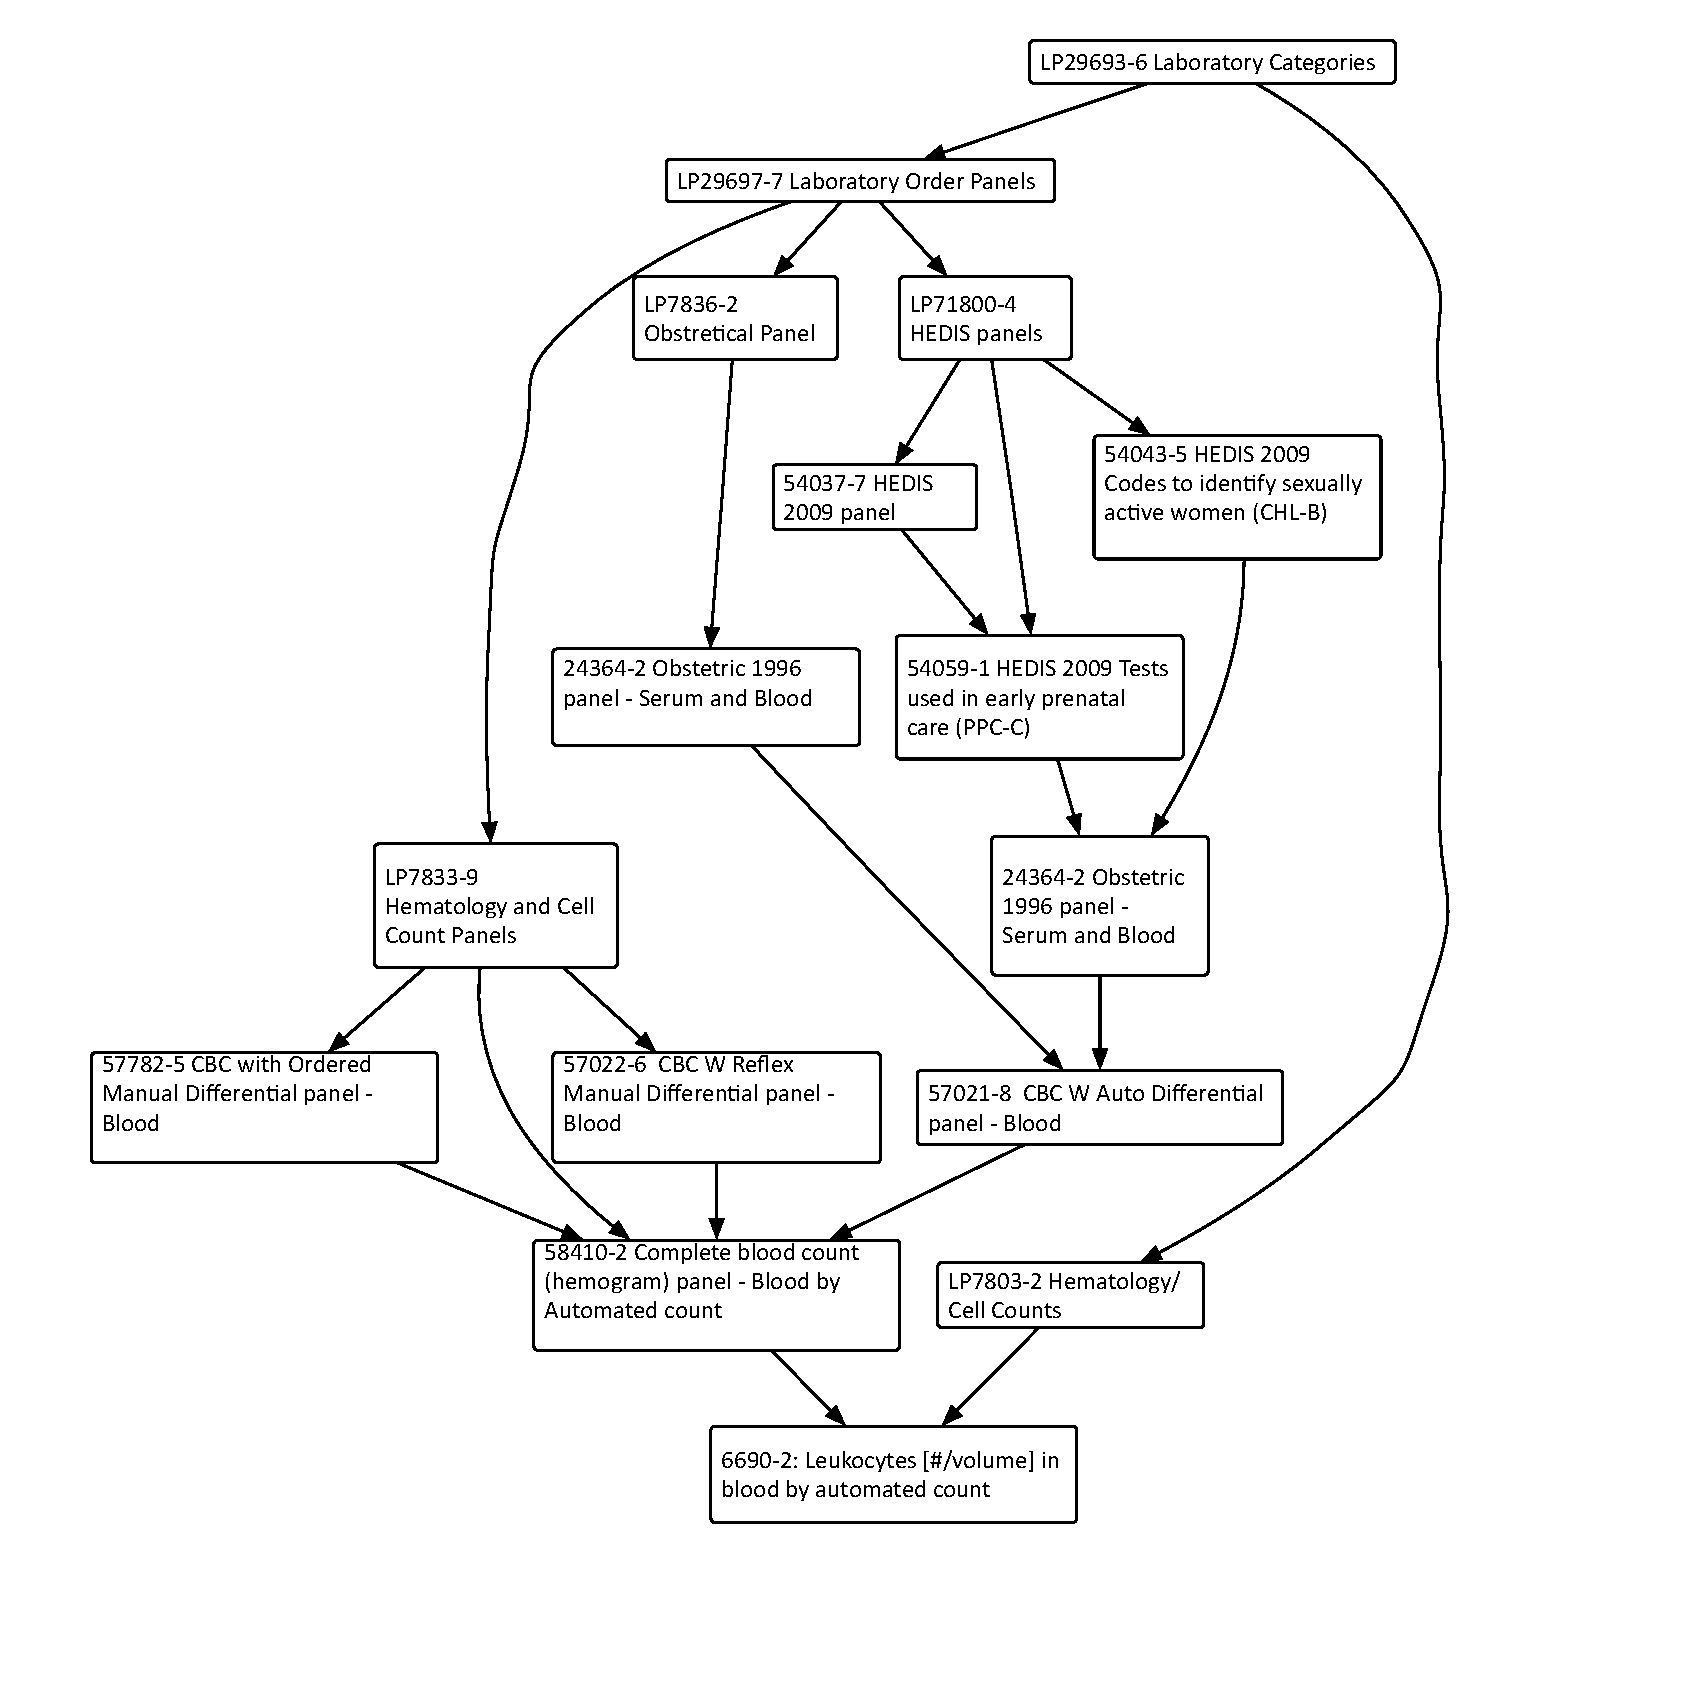
\includegraphics[width=0.59\linewidth, scale=0.5]{diagram1}
		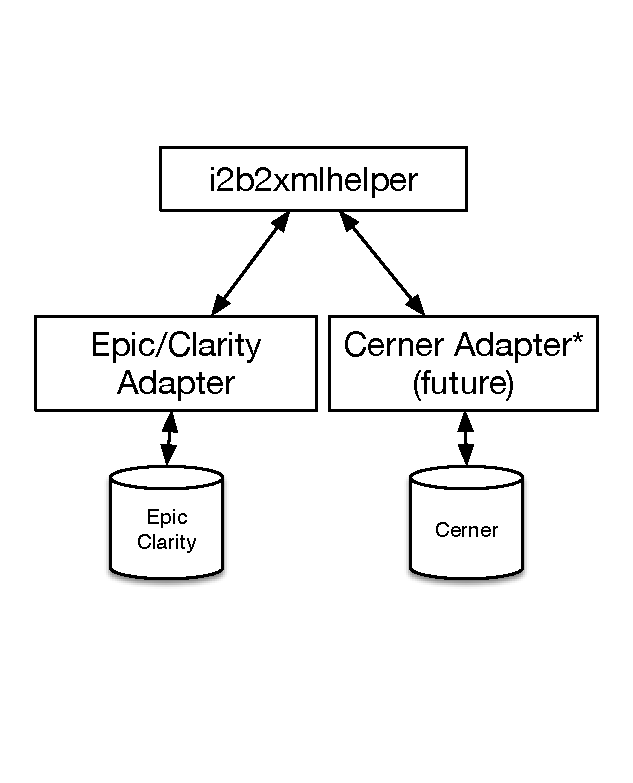
\includegraphics[width=0.5\textwidth]{arch.eps}

	\captionof{figure}{Application architecture}
\end{center}
The application is architected in such a manner that will allow the separation of non-proprietary parts of the code from the vendor specific EMR adapters.  
%----------------------------------------------------------------------------------------
}
\headerbox{Results}{name=results,below=emr, column=2, span=1}{ % To reduce this block to 1 column width, remove 'span=2'

The application has been used to generate over 1,200 \texttt{c\_metadataxml} entries at a selected site. 
\vspace{1em}

If one estimates that to construct a given \texttt{c\_metadataxml} entry manually takes at a minimum 15 minutes, then the time savings garnered from the user of an automated generation tool are quite significant.
%----------------------------------------------------------------------------------------
}
\headerbox{Future work}{name=future,below=results, column=2, span=1}{ % To reduce this block to 1 column width, remove 'span=2'

%----------------------------------------------------------------------------------------
The application needs to have adapters written for other EMR systems to allow a full spectrum of use across the i2b2 community.  Continual refinement of the generated \texttt{c\_metadataxml} entries will be made as experience is gained from its use.
\vspace{1em}

It is anticipated that the code will be placed for use by the community under an open source license.
}
\end{poster}



\end{document}